\documentclass[12pt, a4paper]{report}
\usepackage[
top    = 2.50cm,% presumably you don't want it to be 0pt as well?
bottom = 2.50cm,
left   = 2cm,
right  = 2cm,
marginparsep = 0pt,
marginparwidth=0pt,
]{geometry}
\usepackage{textcomp}
\usepackage{pgfplots}
\usepgfplotslibrary{fillbetween}
\usetikzlibrary{patterns}

\usepackage[export]{adjustbox}
\usepackage{graphicx}
\graphicspath{{pictures/}}
\usepackage{multicol}
\usepackage[siunitx, RPvoltages]{circuitikz}
\usepackage[leqno]{amsmath}
\usepackage[most]{tcolorbox}
\usepackage{varwidth}   %% provides varwidth environmen
\usepackage{amsmath,empheq}
\tcbuselibrary{skins}
\usepackage{cancel}
\newtcolorbox{mybox}[1][]{before=\centering, drop fuzzy shadow, enhanced, colback=white, sharp corners, colframe=red, fonttitle=\bfseries, title=#1, center title}
\setlength{\columnseprule}{1pt}
\usepackage{polynom}
\everymath{\displaystyle}
\makeatletter
\def\pld@CF@loop#1+{%
	\ifx\relax#1\else
	\begingroup
	\pld@AccuSetX11%
	\def\pld@frac{{}{}}\let\pld@symbols\@empty\let\pld@vars\@empty
	\pld@false
	#1%
	\let\pld@temp\@empty
	\pld@AccuIfOne{}{\pld@AccuGet\pld@temp
		\edef\pld@temp{\noexpand\pld@R\pld@temp}}%
	\pld@if \pld@Extend\pld@temp{\expandafter\pld@F\pld@frac}\fi
	\expandafter\pld@CF@loop@\pld@symbols\relax\@empty
	\expandafter\pld@CF@loop@\pld@vars\relax\@empty
	\ifx\@empty\pld@temp
	\def\pld@temp{\pld@R11}%
	\fi
	\global\let\@gtempa\pld@temp
	\endgroup
	\ifx\@empty\@gtempa\else
	\pld@ExtendPoly\pld@tempoly\@gtempa
	\fi
	\expandafter\pld@CF@loop
	\fi}
\def\pld@CMAddToTempoly{%
	\pld@AccuGet\pld@temp\edef\pld@temp{\noexpand\pld@R\pld@temp}%
	\pld@CondenseMonomials\pld@false\pld@symbols
	\ifx\pld@symbols\@empty \else
	\pld@ExtendPoly\pld@temp\pld@symbols
	\fi
	\ifx\pld@temp\@empty \else
	\pld@if
	\expandafter\pld@IfSum\expandafter{\pld@temp}%
	{\expandafter\def\expandafter\pld@temp\expandafter
		{\expandafter\pld@F\expandafter{\pld@temp}{}}}%
	{}%
	\fi
	\pld@ExtendPoly\pld@tempoly\pld@temp
	\pld@Extend\pld@tempoly{\pld@monom}%
	\fi}
\makeatother
\usepackage{wrapfig}
\usepackage{gensymb}
\makeatletter
\let\savedchap\@makechapterhead
\def\@makechapterhead{\vspace*{-3cm}\savedchap}
\usepackage{amssymb}
\usepackage{setspace}
\usepackage[norndcorners,customcolors]{hf-tikz}
\tikzset{set border color=black,set fill color=white}
\newcommand*{\qe}{$x=\frac{-b\pm\sqrt{b^2-4ac}}{2a}$}
\usepackage[linewidth=1pt]{mdframed}
\usepackage{fancyhdr}
\usepackage{array}
\usepackage[utf8]{inputenc}
\usepackage{chngcntr}
\usepackage[english]{babel}
\makeatletter
\newcommand{\leqnomode}{\tagsleft@true\let\veqno\@@leqno}
\newcommand{\reqnomode}{\tagsleft@false\let\veqno\@@eqno}
\makeatother
\usepackage{amsmath}
\usepackage{amsthm}
\theoremstyle{definition}
\newtheorem{example}{Example}
\counterwithin*{example}{section}
\counterwithin*{example}{subsection}
\DeclarePairedDelimiter\abs{\lvert}{\rvert}%
\DeclarePairedDelimiter\norm{\lVert}{\rVert}%

% Swap the definition of \abs* and \norm*, so that \abs
% and \norm resizes the size of the brackets, and the 
% starred version does not.
\makeatletter
\let\oldabs\abs
\def\abs{\@ifstar{\oldabs}{\oldabs*}}
%
\let\oldnorm\norm
\def\norm{\@ifstar{\oldnorm}{\oldnorm*}}
\makeatother
\usepackage{titling}
\predate{}
\postdate{}
\date{} % clear date
\pagestyle{fancy}
\rfoot{\thepage}
\cfoot{}

\setlength{\jot}{13pt}
\begin{document}
	\begin{titlepage} % Suppresses headers and footers on the title page
		
		\centering % Centre everything on the title page
		
		\scshape % Use small caps for all text on the title page
		
		\vspace*{\baselineskip} % White space at the top of the page
		
		%------------------------------------------------
		%	Title
		%------------------------------------------------
		
		\rule{\textwidth}{1.6pt}\vspace*{-\baselineskip}\vspace*{2pt} % Thick horizontal rule
		\rule{\textwidth}{0.4pt} % Thin horizontal rule
		
		\vspace{0.75\baselineskip} % Whitespace above the title
		
		{\LARGE Pure Mathematics\\Advanced Level} % Title
		
		\vspace{0.75\baselineskip} % Whitespace below the title
		
		\rule{\textwidth}{0.4pt}\vspace*{-\baselineskip}\vspace{3.2pt} % Thin horizontal rule
		\rule{\textwidth}{1.6pt} % Thick horizontal rule
		
		\vspace{2\baselineskip} % Whitespace after the title block
		
		%------------------------------------------------
		%	Subtitle
		%------------------------------------------------
		
		“Once your soul has been enlarged by a truth, it can never return to its original size.”\\
		-Blaise Pascal% Subtitle or further description
		
		\vspace*{3\baselineskip} % Whitespace under the subtitle
		
		%------------------------------------------------
		%	Editor(s)
		%------------------------------------------------
		
		Notes By
		
		\vspace{0.5\baselineskip} % Whitespace before the editors
		
		{\scshape\Large Giorgio Grigolo \\ } % Editor list
		
		\vspace{0.5\baselineskip} % Whitespace below the editor list
		
		\textit{Student of Mathematics and Computer Science \\St.Aloysius College } % Editor affiliation
		
		\vfill % Whitespace between editor names and publisher logo
		
		%------------------------------------------------
		%	Publisher
		%------------------------------------------------
		
		
		\vspace{0.3\baselineskip} % Whitespace under the publisher logo
		
		2020 % Publication year
		
	\end{titlepage}
	\tableofcontents
	\newpage
	\chapter{Classification of numbers}
	
	\begin{itemize}
		\item{Natural numbers: $\mathbb{N}$; (1, 2, 3, 4 \ldots)}
		\subitem{This set includes every number which is both positive and whole.}
		\item{Integer numbers: $\mathbb{Z}$; (-2, -1, 0, 1, 2, \ldots)}
		\subitem{The integer number set includes every negative and positive whole numbers, similarly to $\mathbb{N}$}
		\item{Rational numbers: $\mathbb{Q}$; (-1, 2 , $\frac{1}{2}$)}
		\subitem{A number is s.t.b rational if expressed in the form $\frac{p}{q};p, q \in \mathbb{Z}$.}
		\item{Irrational numbers: $\mathbb{Q'}$; ($\pi, e, \sqrt{2}, \sqrt{5}, \ldots$))}
		\subitem{If a number is not classified as any of the above, it is referred to as irrational.}
		\item{Real numbers: $\mathbb{R}$}
		\subitem{Anything mentioned above inclusively represent the set of Real numbers}\\
	\end{itemize}
	
	
	\emph{We can additionally refer to positive or negative numbers in any set by using the notation:}\\
	\begin{center}
		$\mathbb{R}^+$ and $\mathbb{R}^-$
	\end{center}
	%TODO: insert image of sets
	
	
	\newpage
	\chapter{Surds}
	\section{Introduction}
	\quad Consider numbers $\sqrt{64}, \sqrt{16}$. These can be represented as exact quantities by writing $8$ and $4$. There are however other numbers which cannot be expressed as exact quantities using other symbols.\\
	
	
	There is an option of expressing them as corrected decimals without however preserving their full value. Instead, we choose to keep the form $\sqrt{a}$ which preserves the full value of the numbers.
	\section{Examples}
	\begin{multicols}{2}
		\noindent
		\begin{alignat*}{2}
			a)\quad
			\sqrt{2} & = \sqrt{16\times3}          \\
			& = \sqrt{16} \times \sqrt{3} \\
			& = 4\sqrt{3}                 
		\end{alignat*}
		\begin{alignat*}{2}
			b)\quad
			\sqrt{72} & = \sqrt{8\times9}         \\
			& = \sqrt{9}\times \sqrt{8} \\
			& = 3\sqrt{8}               
		\end{alignat*}
		\begin{alignat*}{2}
			\quad
			\sqrt{360} & = \sqrt{180} \times \sqrt{2} \\
			& =\sqrt{36}\times\sqrt{10}    \\
			& =6\sqrt{10}                  
		\end{alignat*}
		\begin{alignat*}{2}
			d)\quad
			& \quad\left(1+2\sqrt{3}\right)\left(2+3\sqrt{5}\right) \\
			& = 2-\sqrt{3}  - 10\sqrt{3}                            \\
			& =-28-\sqrt{3}                                         
		\end{alignat*}
		\begin{alignat*}{2}
			e)\footnote[1]\quad
			& \quad\left(2-3\sqrt{5}\right)\left(2+3\sqrt{5}\right) \\
			& = 4+6\sqrt{5}-6\sqrt{5}-9(5)                          \\
			& =-41                                                  
		\end{alignat*}
	\end{multicols}
	\footnotetext[1]{This expression shows that for products of the form $\left(a+b\sqrt{c}\right)\left(a-b\sqrt{c}\right)$ the surds will vanish.}
	\newpage
	\section{Rationalizing the denominator}
	\quad \emph{Consider the fraction:} 
	$$\frac{1}{1+\sqrt{2}}$$
	This fraction contains a surd, thus, making it irrational. To rationalize said fraction one should find the multiplicative operation of canceling the denominator \textit{(see \footnotemark[1])}.\\
	
	
	\emph{Continuing...}
	\begin{alignat*}{2}
		\frac{1}{1+\sqrt{2}} & = \frac{1}{1+\sqrt{2}} \times \frac{1-\sqrt{2}}{1-\sqrt{2}} \\
		& =\frac{1-\sqrt{2}}{1}                                       \\
		& =1-\sqrt{2}                                                 
	\end{alignat*} 
	
	
	\chapter{Partial Fractions}
	\section{Introduction}
	\emph{Consider the expression and suppose it is simplified:}
	
	
	\begin{alignat*}{2}
		\frac{2}{x+1}+\frac{3}{2x-5} & = \frac{2(2x-5)+3(x+1)}{(x+1)(2x-5)} \\
		& =\frac{4x-10+3x+3}{(x+1)(2x-5)}      \\
		& =\frac{4x-10+3x+3}{(x+1)(2x-5)}      \\
		& =\frac{7x-7}{(x+1)(2x-5)}            \\
	\end{alignat*}
	
	In this chapter we reverse the approach above, hence decomposing one fraction to its corresponding partial fractions.
	\newpage
	\section{Types of partial fraction cases}
	\subsection*{\underline{Type 1: Linear Factors in denominator}}
	\begin{example}
		Decompose $ \frac{7x-7}{\left(x+1\right)}$ into Partial Fractions
	\end{example}
	\begin{alignat*}{2}	
		&            & \frac{7x-7}{\left(x+1\right)} & \equiv \frac{A}{\left(x+1\right)} + \frac{B}{\left(2x-5\right)} \\
		& \implies   & 7x-7                          & = A\left(2x-5\right)+B\left(x+1\right))                         \\	
		& \implies   & 7(-1)-7                       & = A(2(-1)-5)\tag*{$x = -1$}                                     \\
		& \implies   & -14                           & = -7A                                                           \\\leqnomode
		& \implies   & A                             & = 2\tag{..1}                                                    \\
		& \implies   & 7\left(\frac{5}{2}\right)-7   & =B\left(\left(\frac{5}{2}\right)+1\right)\tag*{$x=\frac{5}{2}$} \\
		& \implies   & \frac{35}{2} - 7              & = \frac{7B}{2}                                                  \\
		& \implies   & B                             & =3\tag{..2}                                                     \\\\
		& \therefore & \frac{7x-7}{\left(x+1\right)} & = \frac{2}{\left(x+1\right)} + \frac{3}{\left(2x-5\right)}      
	\end{alignat*}
	
	
	\subsection*{\underline{Type 2: Irreducible Quadratic Factor in Denominator}}
	\begin{example}
		Decompose $\frac{x^2 +1}{(2x+1)(x^2 +3)}$ into its corresponding partial fractions.
	\end{example}
	\begin{alignat*}{2}
		&            & \frac{x^2 +1}{(2x+1)(x^2 +3)} & \equiv \frac{A}{2x+1}+\frac{Bx+C}{x^2 +3}       \\
		& \implies   & x^2 + 1                       & \equiv A(x^ 2 + 3) + (Bx+C)(2x+1)               \\
		& \implies   & x^2 + 1                       & \equiv x^2(A+2B) + x(2B + 2C) + (3A+C)\tag{*..} \\
		\intertext{\quad At this stage, since both equations are identical, we analyse the different coefficients and constants to form a system of equations to solve.}
		\intertext{Comparing coefficients of $x^2\colon$}
		&            & 1                             & = A+2B\tag{1..}                                 \\
		\intertext{Comparing coefficients of $x\colon$}
		&            & 0                             & = B+C\tag{2..}                                  \\
		\intertext{Comparing constants$\colon$}
		&            & C                             & = 1-3A\tag{3..}                                 \\
		\intertext{Substituting  3.. in 2..}
		&            & 0                             & =B+1-3A                                         \\
		& \implies   & B                             & =3A-1\tag{4..}                                  \\
		\intertext{Substituting 4.. in 1..}
		&            & 1                             & = A + 2(3A-1)                                   \\
		& \implies   & A                             & = \frac{-1}{7} \tag{5..}                        \\
		\intertext{Substituting 5.. in 1..}
		&            & 1                             & = \frac{-1}{7} +2B                              \\
		& \implies   & -7                            & = 1-14B                                         \\
		& \implies   & B                             & =\frac{4}{7}\tag{6..}                           \\
		\intertext{Substituting 5.. in 3..}
		&            & C                             & = 1-3\left(\frac{-1}{7}\right)                  \\
		& \implies   & C                             & = \frac{10}{7}                                  \\
		& \therefore & \frac{x^2 +1}{(2x+1)(x^2 +3)} & \equiv \frac{A}{2x+1}+\frac{Bx+C}{x^2 +3}       
	\end{alignat*}
	\newpage
	\subsection*{\underline{Type 3: Repeated factor in the denominator}}
	\begin{example}
		Decompose $\frac{x+1}{(x+2)(x-3)^2}$ into its corresponding partial fractions.
	\end{example}
	\begin{alignat*}{2}
		&            & \frac{x+1}{(x+2)(x-3)^2} & \equiv \frac{A}{x+2} + \frac{B}{x-3} + \frac{C}{(x-3)^2}           \\
		& \implies   & x+1                      & \equiv A(x-3)^2 + B(x-3)(x+2) + C(x+2)                             \\
		& \implies   & x+1                      & \equiv Ax^2 - 6Ax +9A + Bx^2-Bx-6B + Cx+2C)                        \\
		& \implies   & -2+1                     & =A(-2-3)^2\tag*{$x=-2$}                                            \\
		& \implies   & A                        & = \frac{-1}{25}                                                    \\
		& \implies   & 3+1                      & =C(3+2)\tag*{$x=3$}                                                \\
		& \implies   & C                        & =\frac{4}{5}                                                       \\
		\intertext{Comparing coefficients of $x^2\colon$}
		& \implies   & 0                        & = A + B                                                            \\
		& \implies   & B                        & = \frac{1}{25}                                                     \\
		& \therefore & \frac{x+1}{(x+2)(x-3)^2} & \equiv \frac{1}{25(x-3)} + \frac{4}{5(x-3)^2} - \frac{-1}{25(x-3)} \\
	\end{alignat*}
	
	The approach above, is similar to the previous one, with the addition of the fact that each repeated factor has to be listed in order of powers until its own.
	\newpage
	\subsection*{\underline{Type 4: Improper fraction}}
	\begin{example}
		Decompose $\frac{2x^2 -8x +11}{2x-5}$ into its corresponding partial fractions.
	\end{example}
	Since the fraction is improper, or top-heavy\footnotemark[2] it is required to perform a polynomial long division and acquire the proper terms. \footnotetext[2]{Improper fractions containing a variable are recognized by the order of the exponent when the expression is expanded. i.e $\frac{x^2}{x+5}$ is regarded as improper}
	\begin{center}
		\polylongdiv{2x^2 -8x +11}{2x-5}
	\end{center}
	\begin{alignat*}{2}
		& \therefore\quad & \frac{2x^2 -8x +11}{2x-5} & \equiv 	x - \frac{3}{2} + \frac{7}{2(2x-5)} 
	\end{alignat*}
	\newpage
	\chapter{Pascal's Triangle}
	\bigskip
	\emph{Consider the following expansions:}
	\begin{gather*}
		(1+x)^0 = 1\\
		(1+x)^1 = 1+x\\
		(1+x)^2 = 1+2x+x^2\\
		(1+x)^3 = 1+3x+3x^2+x^3\\
		(1+x)^4 = 1+4x+6x^2+4x^3+x^4\\
		(1+x)^5 = 1+5x+10x^2+10x^3+5x^4+x^5\\
		(1+x)^6 = 1+6x+15x^2+20x^3+15x^4+6x^5+x^6\\
		\ldots\\
		\begin{tabular}{>{$n=}l<{$\hspace{12pt}}*{13}{c}}
			&   &   &   &   &    &    & 1  &    &    &   &   &   &   \\
			&   &   &   &   &    & 1  &    & 1  &    &   &   &   &   \\
			&   &   &   &   & 1  &    & 2  &    & 1  &   &   &   &   \\
			&   &   &   & 1 &    & 3  &    & 3  &    & 1 &   &   &   \\
			&   &   & 1 &   & 4  &    & 6  &    & 4  &   & 1 &   &   \\
			&   & 1 &   & 5 &    & 10 &    & 10 &    & 5 &   & 1 &   \\
			6 & 1 &   & 6 &   & 15 &    & 20 &    & 15 &   & 6 &   & 1 
		\end{tabular}
	\end{gather*}\\
	The above array of numbers is called Pascal's Triangle. It can be used to expand any binomial. The following examples illustrate its use.\\
	\newpage
	\begin{example}
		Expand the following using Pascal's Triangle
	\end{example}
	\begin{alignat*}{2}
		(1+2x)^5                      & \equiv 1(2x)^0 + 5(2x)^1 + 10(2x)^2 + 10(2x)^3 + 5(2x)^4 + 2x^5\tag*{a)}                                                                          \\
		& \equiv 1 + 10x + 40x^2 + 80x^3 + 80x^4 + 32x^5                                                                                                    \\
		\\	
		\left(1-\frac{3x}{2}\right)^6 & \equiv 1\left(\frac{-3x}{2}\right)^0 + 6\left(\frac{-3x}{2}\right)^1 + 15\left(\frac{-3x}{2}\right)^2 + 20\left(\frac{-3x}{2}\right)^3 +\tag*{b)} \\
		& \quad 15\left(\frac{-3x}{2}\right)^4 + 6\left(\frac{-3x}{2}\right)^5 + 1\left(\frac{-3x}{2}\right)^6                                              \\
		& \equiv 1 - 9x + \frac{135x^2}{4} - \frac{135x^3}{2} + \frac{1215x^4}{16} - \frac{243x^5}{16} + \frac{728x^6}{64}                                  \\
		&   \\(p+q)^4 &\equiv (p(1+\frac{q}{p}))^4\tag*{c)}\\
		& \equiv p^4\left(1+\frac{q}{p}\right)^4                                                                                                            \\
		& \equiv p^4\left(1 + \frac{4q}{p} + \frac{6q^2}{p^2} + \frac{4q^3}{p^3} + \frac{q^4}{p^4}\right)                                                   \\
		& \equiv p^4 + 4p^3q + 6p^2q^2 + 4pq^3 + q^4                                                                                                        
	\end{alignat*}
	In the above examples we observe that: 
	
	\begin{itemize}
		\item{The expansion contains the coefficients for Pascal's Triangle.}
		\item{The expansion is formed by descending exponents of the first term of the binomial \& ascending exponents of the second.}
		\item{The sum of the exponents in each term is equal to the 	exponent by which the binomial was raised.}
	\end{itemize}
	These observations can be applied to expand any binomials raised with positive integer exponents.
	\newpage
	\chapter{The Remainder and Factor Theorems}
	\section{The Remainder Theorem}
	Consider the polynomial $f(x)$. Suppose that this polynomial is to be divided by the linear expression $x-a$. This gives:
	\begin{alignat*}{3}
		&&\frac{f(x)}{x-a}A&\equiv Q(x) + \frac{R}{x-a}\\
		&\implies&f(x) &\equiv Q(x) \cdot (x-a) + R\\
		\text{Let $x-a=0$}&\implies &x &= a\\
		& \therefore & f(a) & = R;\quad & \text{Where R is the remainder of $\frac{f(x)}{x-a}$} \\
		&            &      &           & \text{and Q is the quotient of $\frac{f(x)}{x-a}$}    \\
	\end{alignat*} \\
	\begin{example}
		Find the remainder when the cubic polynomial $f(x) = 2x^3-3x-5$ is divided by $x-2$
	\end{example}
	
	
	If $f(x)$ is to be divided by $x-2$, then $f(2)$ is equal to the remainder of $\frac{2x^3-3x-5}{x-2}$
	\begin{alignat*}{2}
		&        & 2x^3 -3x-5       \\
		& =\quad & 2(2)^3 - 3(2) -5 \\
		&\boxed{\therefore\quad R\quad=\quad5}
	\end{alignat*}
	\section{The Factor theorem}
	
	The factor theorem states that:
	\begin{itemize}
		\item{If the polynomial $f(x)$ is divided by $x-a$, then $f(a) = 0$ (i.e $R=0$}), therefore it can also be concluded that $x-a$ is a factor of $f(x)$
	\end{itemize}
	\begin{example}
		Determine whether $2x+3$ is a factor of $2x^3+x^2-5x+6$ 
	\end{example}
	
	\begin{flalign*}
		&  & \text{Let } f(x) &= 2x^3+x^2-5x+6& \\
		& \rlap{If $2x+3$ is a factor of $f(x)\colon$} &0 &=f\left(\frac{-3}{2}\right)\\
		&\rlap{However,} &0 &\neq 2\left(\frac{-3}{2}\right)^3 + \left(\frac{-3}{2}\right)^2 -5\left(\frac{-3}{2}\right) + 6 \\
		&&&\neq -3\\
		&&&\boxed{\therefore \quad \text{$2x+3$ is \textbf{not} a factor of $f(x)$}}
	\end{flalign*}
	\newpage
	\chapter{Quadratic Equations}
	\section{Definition}
	\quad A quadratic equation is of the form $ax^2+bx+c=0$ where $a,b,c \in \mathbb{R},\quad a\neq0$. These can be solved algebraically using one of the following methods:
	\begin{itemize}		
		\item{Fractions}
		\item{Completing the square}
		\item{The quadratic formula\footnote[3]{\qe}}
	\end{itemize}
	\section{Nature of roots of the Quadratic Equation}
	\quad Any quadratic equation has in general two roots, namely \qe.
	The quantity $b^2-4ac$ determines the nature of these roots.
	\begin{itemize}
		\item{$b^2-4ac > 0\colon$ Equation holds two real and distinct roots.}
		\item{$b^2-4ac = 0\colon$ Equation holds two equal\footnote[4]{It is implied that they are real.} roots.}
		\item{$b^2-4ac > 0\colon$ Equation holds two complex roots.}
	\end{itemize}
	\quad Thus, the quantity $b^2-4ac$ discriminates among the type of roots that a quadratic equation may have. Therefore it is called the discriminant.
	\begin{example}
		Determine, without solving the nature of the following function.
	\end{example}
	\begin{alignat*}{2}
		& Let        & f(x) =                 & 2x^2+3x-17                              \\
		& \implies   & b^2-4ac                & =3^2-4(2)(-17)                          \\
		&            &                        & = 145                                   \\
		&            &                        & > 0                                     \\
		& \therefore & \text{Roots of $f(x)$} & \in \mathbb{R} \text{ and are distinct} 
	\end{alignat*}
	\hrulefill
	\begin{example}
		Determine the value of $p$ if $ px^2-10x+1 = 0 $ has two equal roots
	\end{example}
	
	Given that the equation has two equal roots:
	
	\begin{alignat*}{2}
		&          & b^2-4ac                        & = 0 \\
		& \implies & 100-4p                         & = 0 \\
		&          & \boxed{\therefore \quad p = 5} &     
	\end{alignat*}
	
	\newpage
	\section{Roots and Coefficients of a Quadratic Equation}
	\subsection{Proof}
	\emph{Consider a general quadratic equation:}
	\begin{alignat*}{2}
		&            & ax^2+bx+c                            & = 0 \tag{1..}                              \\
		& \implies   & x^2 +\frac{bx}{a} + \frac{c}{a}      & = 0                                        \\
		\intertext{Let $\alpha$  and $\beta$  be the roots:}
		& \implies   & (x-\alpha)(x-\beta)                  & = 0                                        \\
		& \implies   & x^2 -\beta x -\alpha x + \alpha\beta & = 0                                        \\
		& \implies   & x^2-(\alpha + \beta)x + \alpha\beta  & = 0\tag{2..}                               \\
		\intertext{Since (1..) and (2..) are identical:}
		& \implies   & x^2 +\frac{bx}{a} + \frac{c}{a}      & \equiv x^2-(\alpha + \beta)x + \alpha\beta \\
		& \therefore & \alpha + \beta                       & = \frac{-b}{a}                             \\ 
		&            & \alpha\beta                          & = \frac{c}{a}                              
	\end{alignat*}
	\hrulefill
	
	\begin{example}
		Write down the quadratic equation whose roots have a sum of 7 \& a product of 5.
	\end{example}
	\begin{alignat*}{2}
		&   &        & x^{2} - (\alpha + \beta) + (\alpha\beta) \\
		&   & =\quad & x^2 - 7x + 7                             
	\end{alignat*}
	\hrulefill
	\begin{example}
		The roots of the equation $2x^2 + 5x -1$ are $\alpha$ and $\beta$. Find the equation whose roots are $\frac{1}{\alpha} $ \& $\frac{1}{\beta}$
	\end{example}
	\begin{alignat*}{2}
		&   & \alpha + \beta & = \frac{-5}{2} \\
		&   & \alpha\beta    & = \frac{-1}{2} 
	\end{alignat*}
	\newpage
	\begin{multicols}{2}
		\textit{Sum of roots:}
		\begin{alignat*}{2}
			&   &   & \frac{1}{\alpha} + \frac{1}{\beta} \\
			&   & = & \frac{\alpha+\beta}{\alpha\beta}   \\
			&   & = & \frac{-5}{2} \div \frac{-1}{2}     \\
			&   & = & 5                                  
		\end{alignat*}
		\textit{Product of roots:}
		
		\begin{alignat*}{2}
			\\&&&\frac{1}{\alpha\beta}\\
			&   & = & \frac{-2}{1} \\
			&   & = & -2           
		\end{alignat*}
	\end{multicols}
	\[ 
	\therefore \quad f(x) = x^2-5x-2
	\]
	\newpage
	\chapter{Logarithms}\label{sec:logarithms}
	\section{Definition}
	\quad In mathematics, the logarithm is the inverse function to exponentiation. That means the logarithm of a given number $x$ is the exponent to which another fixed number, the base $b$, must be raised, to produce that number $x$.\\
	
	\emph{Consider: }\\$$ 2^3 = 8$$\\
	
	3 is the exponent by which 2 must be raised to obtain 8. This statement can also be reversed:\\ 3 is the logarithm by which with a base of 2, results in 8. Thus:$$ 3 = \log_28$$\\
	
	\emph{In general: }\\$$a^b = c \iff \log_ac = b ,\quad a \in \mathbb{R^+}$$\\
	
	
	Furthermore, it is standard to represent $\log_{10}(x)$ as $\log(10) $ and $ \log_e(x) $ as $ \ln(x) $
	
	
	\bigskip
	\bigskip
	\bigskip
	\bigskip
	
	\tcbset{
		enhanced,
		colback=red!5!white,
		boxrule=0.1pt,
		colframe=black!75!black,
		fonttitle=\bfseries
	}
	\begin{center}
		\begin{tcolorbox}[center title,hbox,    %%<<---- here
			lifted shadow={1mm}{-2mm}{3mm}{0.1mm}%
			{black!50!white}]
			\begin{varwidth}{\textwidth}
				\begin{center}
					$	\log_a1                         = 0                    $ \\
					\bigskip
					$\log_aa                          = 1                    $ \\
					\bigskip
					$	\log_c(ab)                       \equiv \log_ca + log_cb $\\
					\bigskip
					$	\log_c\left (\frac{a}{b}\right)  \equiv \log_ca - log_cb$ \\
					\bigskip
					$	n\log_ca                         \equiv \log_ca^n   $     
				\end{center}
			\end{varwidth}
		\end{tcolorbox} 
	\end{center}
	\section{Proofs}
	
	
	
	\paragraph{Proof 1: }$\log_aa  = 1$
	\begin{center}
		$	\text{Let} \log_aa = x$
		$$   a^x      = a $$
		$$x        =1 $$
	\end{center}
	\paragraph{Proof 2: }$\log_aa  = 1$
	\begin{center}
		$	\text{Let} \log_a1 = x$
		$$   a^x      = 1 $$
		$$x        = 0$$
	\end{center}
	\paragraph{Proof 3: }$\log_cab  = \log_ca + \log_cb$
	\begin{center}
		$	\text{Let} \log_ca = x$ ; $\text{Let} \log_cb = y$
		$$\Rightarrow  c^{x} = a  \text{ ; } c^{y} = b$$
		$$\Rightarrow ab = c $$
		$$\Rightarrow\log_c(ab) = \log_c(x) + \log_c(y)$$
		$$\therefore\quad \log_c(ab) = \log_c(a) + \log_c(b)$$
	\end{center}
	\paragraph{Proof 4: }$\log_c\frac{a}{b}  = \log_ca - \log_cb$
	\begin{center}
		$	\text{Let} \log_ca = x$ ; $\text{Let} \log_cb = y$
		$$  c^{x} = a  \text{ ; } c^{y} = b$$
		$$\frac{a}{b} = c^x \times c^{-y} $$
		$$\log_c\frac{a}{b} = \log_c(x) - \log_c(y)$$
	\end{center}
	\paragraph{Proof 5: }$\log_ca^n = n\log_ca$
	\begin{center}
		$	\text{Let} \log_ca^n = x$
		$$ c^x = a^n$$
		$$c^{\frac{x}{n}} = a  $$
		$$\log_ca = \frac{x}{n}$$
		$$x = n\log_ca $$
	\end{center}
	\chapter{Vectors}
	\section{Definition}
	\quad A vector quantity is one which has magnitude and direction. For example, length is defined only by size and therefore is a \textit{scalar quantity}. However, acceleration due to gravity, while having a known magnitude, it is also acting in a particular direction. Hence, acceleration is a vector quantity.
		
\begin{wrapfigure}{r}{0.25\textwidth}
	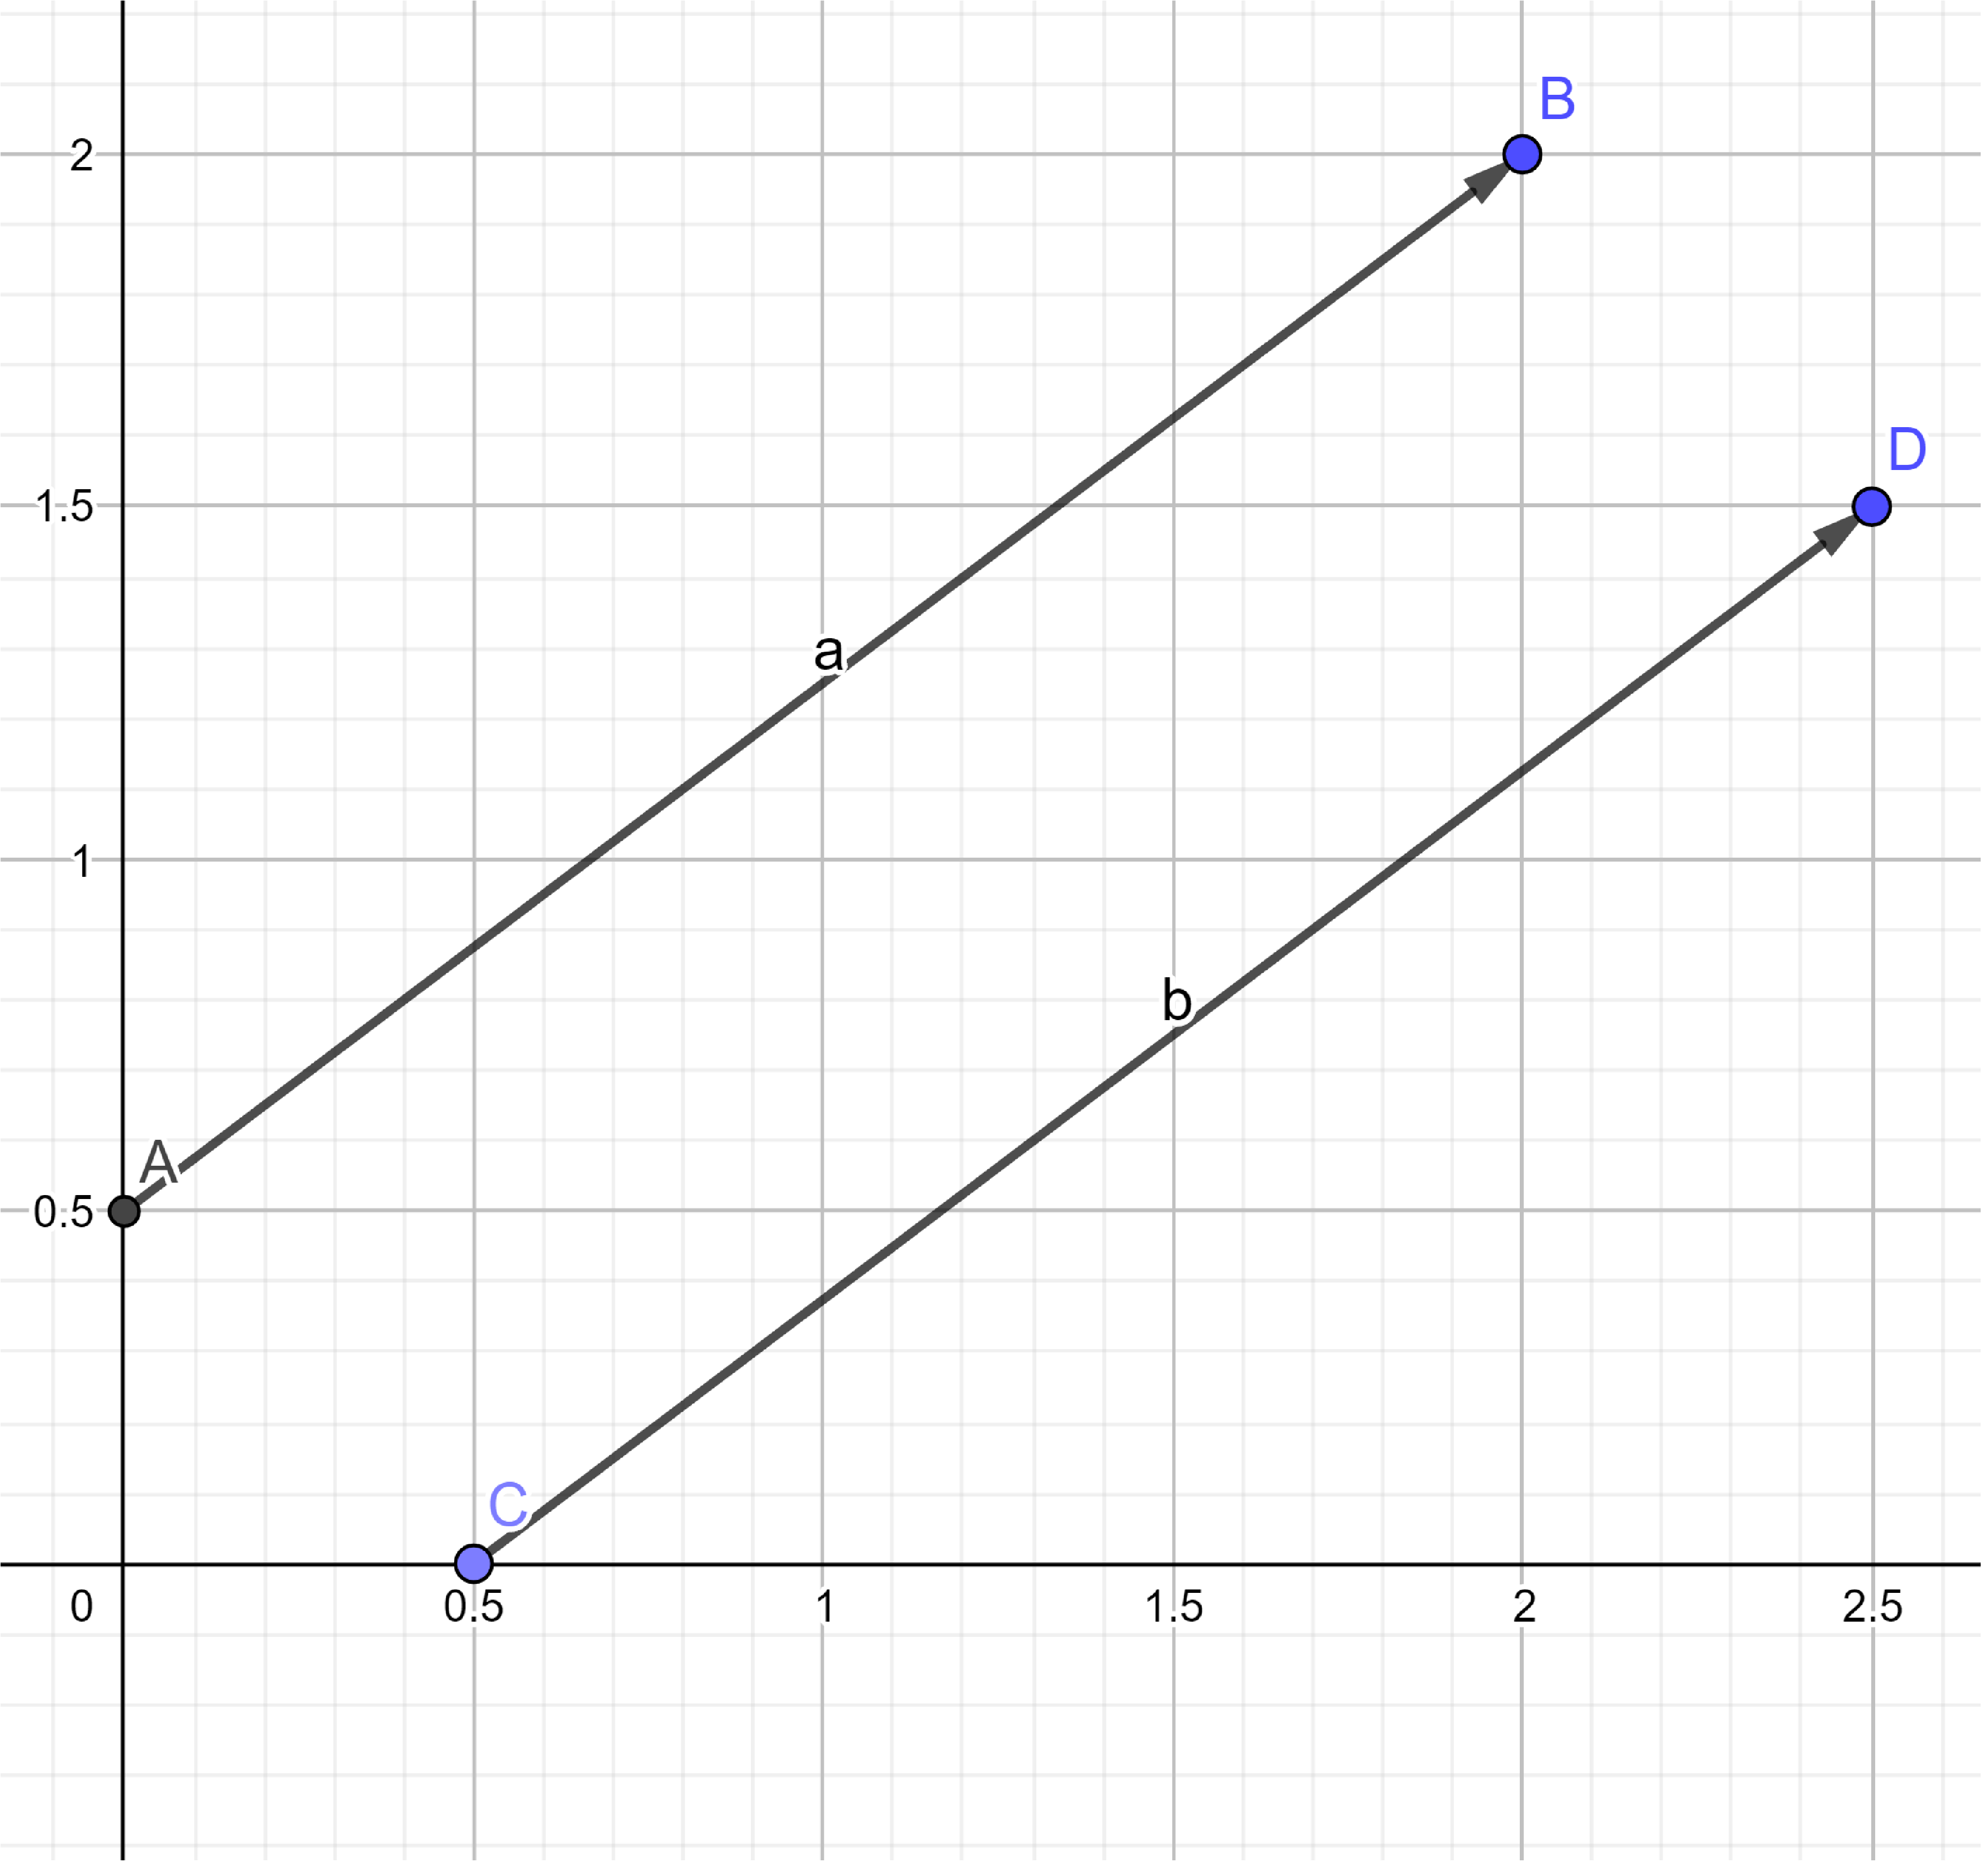
\includegraphics[width=1.3\linewidth]{vect_1} 
\end{wrapfigure}

Vectors are represented using line segments with arrows to denote their direction. Hence, we may consider vector $\overrightarrow{AB}$.

\begin{itemize}
	\item{Two vectors are s.t.b equal iff they have the same magnitude and act in the same direction.}
	\item{The modulus refers to the size of a vector $\underline{a}$ and is denoted by $\abs{a}$.}
	\item{Two vectors $\underline{a}$ and  $-\underline{a}$  are equal in magnitude but opposite in direction. Hence the negative sign indicates opposing direction.}
	\item{When a vector is multiplied by a scalar, its magnitude changes. thus $\lambda  \underline{a}$ is a vector in the same direction as  $\underline{a}$ but has magnitude $\lambda\abs{\underline{a}}$}
\end{itemize}
	\section{Position Vectors and Free Vectors}
	\quad When we refer to a vector  $\underline{a}$ we refer to a vector which is not confined to a specific position on the plane or in space.  $\underline{a}$, as such, is a \textit{free vector}.\\
	
	 When we refer to the position vector  $\underline{b}$, we refer to a vector which is initially set to start from a specific location, usually, the origin.\\
		\begin{wrapfigure}{l}{0.25\textwidth}
		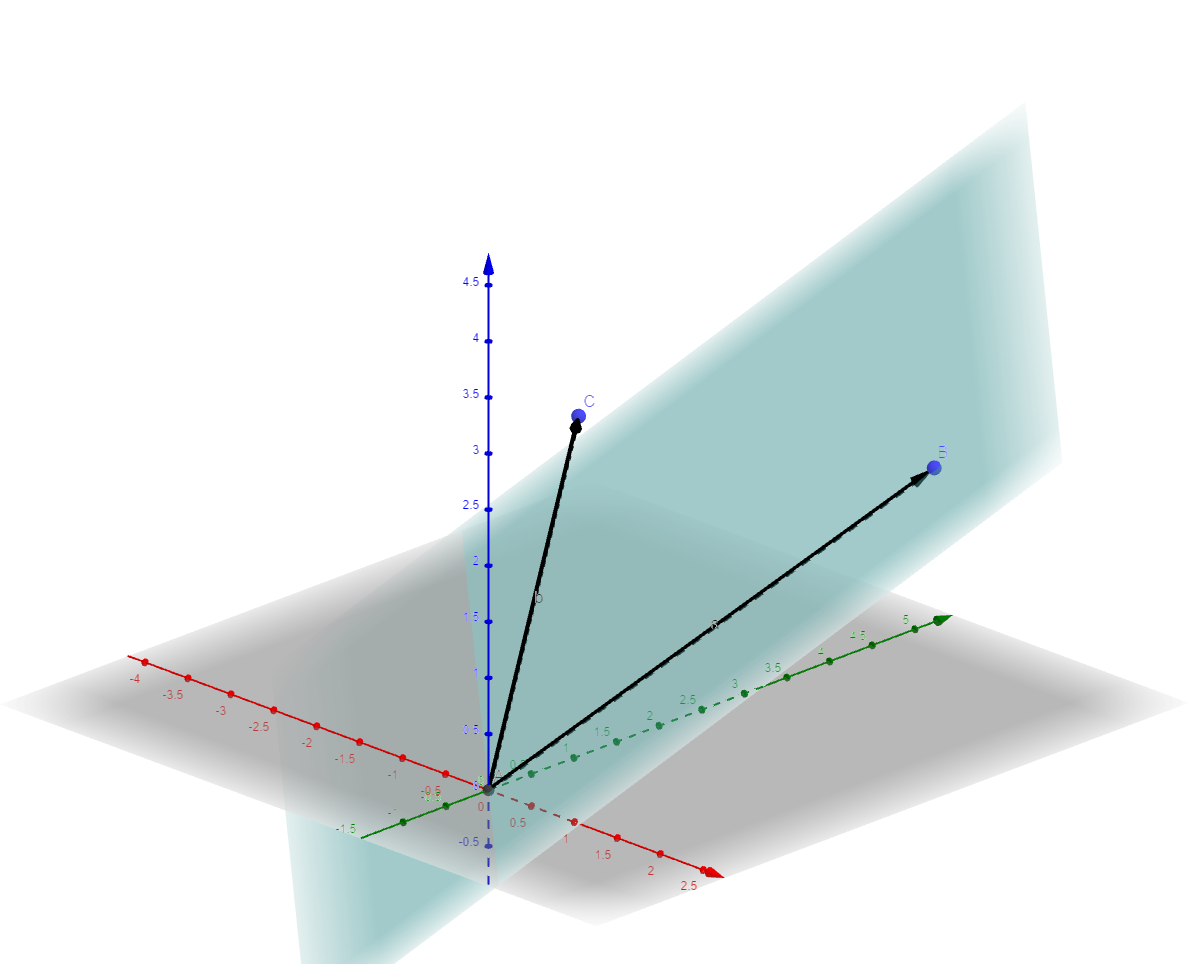
\includegraphics[width=1.3\linewidth]{vect_2} 
	\end{wrapfigure}
	 Suppose that  $\underline{a}$ and  $\underline{b}$ are non-parallel free vectors, and that the origin is a fixed point. There exists only one plane which contains the point $(0,0)$,  $\underline{a}$ and  $\underline{b}$.
	 

	

	\newpage
	\chapter{Inequalities}
	\section{Quadratic Inequalities}
	\begin{example}
		Solve the inequality $x^2-2x>3$
	\end{example}
	
	\begin{center}
		$$x^2-2x>3$$
		$$\implies x^2-2x-3>0$$
		$$\text{Let }x^2-2x-3=0$$
		$$\implies(x-3)(x+1)=0$$
	\end{center}	
	\begin{center}
		\begin{tikzpicture}
			\begin{axis}[
				width=8cm,
				height=6cm,
				axis line style={-},
				xmin=-4,
				xmax=4,
				ymin=-4,
				ymax=5,
				xtick={-1,3}, % remove all ticks from x-axis
				ytick={-3}, % ditto for y-axis
				xlabel=$x$, 
				ylabel=$y$,
				axis lines=center, % default is to make a box around the axis
				samples=100]
				\addplot [black] {x^2 - 2*x - 3}
				;
			\end{axis}
		\end{tikzpicture}
	\end{center}
	\hrulefill
	\begin{example}
		Solve the inequality $\quad \dfrac{2x^2}{5} \leq \dfrac{7x+10}{2}$
	\end{example}
	\begin{center}
		$$4x^2 \leq 35x + 50$$
		$$\implies 4x^2-35x-50\leq 0$$
		$$\text{Let }\quad 4x^2-35x-50=0$$
		$$(4x+5)(x-10)=0$$
		\begin{tikzpicture}
			\begin{axis}[
				width=8cm,
				height=6cm,
				axis line style={-},
				xmin=-2,
				xmax=11,
				ymin=-127,
				ymax=50,
				xtick={-5/4,10}, 
				ytick={-50}, 
				xlabel=$x$, 
				ylabel=$y$,
				axis lines=center, 
				samples=100]
				\addplot [black] coordinates{
					(-1,-17)(0,-48)(1,-79)(2,-110)(3,-141)(4,-172)(5,-203)(6,-234)(7,-265)(8,-296)(9,-327)(10,-358)(11,-389)	
				};
			\end{axis}
		\end{tikzpicture}
	\end{center}
	
	\hrulefill
	
	
	
	
	\chapter{Series}
	\section{Maclaurin Series}
	\subsection{Derivation}
	Let $f(x)$ be nay function of $ x $ and suppose that $ f(x) $ can be expanded as a series of ascending powers of $ x $ and that this series can be differentiated $ w.r.t. x $
	\begin{center}
		$	f(x) \equiv a_0   + a_{1}x  + a_{2}x^2 + a_{3}x^3 + a_{4}x^4 + ... +	 a_{r}x^r$\\
		\text{where $a_n$ are constants to be found}
	\end{center}
	Thus, inputting $0$ into $f(x)$ returns:
	$$\boxed{f(0) = a_{0}}$$\\
	Differentiating  $f(x)$ $w.r.t.x\colon$ 
	$$f'(x) \equiv a_{1} + 2a_{2}x + 3a_{3}x^2 + 4a_4x^3 + \cdots + ra_{r}x^{r-1} + \cdots$$
	Inputting $0$ into $f'(x)\colon$
	$$\boxed{f'(0) = a_1}$$\\
	Differentiating $f'(x)$ $w.r.t.x\colon$
	$$f''(x) \equiv 2a_{2} + 6a_{3}x + 12a_4x^2 + \cdots + (r-1)(r)a_{r}x^{r-2} + \cdots$$
	Inputting $0$ into $f''(x)\colon$
	$$\boxed{f''(0) = 2a_2}$$\\
	Differentiating $f''(x)$ $w.r.t.x\colon$
	$$f'''(x) \equiv 6a_{3} +24a_4x + \cdots + (r-2)(r-1)(r)a_{r}x^{r-3}+ \cdots$$
	Inputting $0$ into $f'''(x)\colon$
	$$\boxed{f'''(0) = (2)(3)a_3}$$
	$$\vdots$$
	\newpage
	By the above calculation we can conclude that: 
	$$\boxed{a_r = \frac{f^r(x)}{r!}}$$
	Considering all of the above: 
	
	\tcbset{
		enhanced,
		colback=red!5!white,
		boxrule=0.1pt,
		colframe=black!75!black,
		fonttitle=\bfseries
	}
	\begin{center}
		\begin{tcolorbox}[center title,hbox,    %%<<---- here
			lifted shadow={1mm}{-2mm}{3mm}{0.1mm}%
			{black!50!white}]
			\begin{varwidth}{\textwidth}
				\begin{center}
					$f(x) \equiv f(0) + f'(0)x + \dfrac{f''(0)x^2}{2!} + \dfrac{f'''(0)x^3}{3!} + \cdots + \dfrac{f^r(0)x^r}{r!} + \cdots$\\
					\bigskip
					$\displaystyle \therefore \quad f(x) \equiv \sum_{r=1}^{\infty} \dfrac{f^r(x)}{r!}$
				\end{center}
			\end{varwidth}
		\end{tcolorbox} 
	\end{center}
	
	
	This is known as Maclaurin's Theorem, and can be obtained if and only if $f^r(0) \in \mathbb{R}$. In the following examples we use Maclaurin's Theorem to obtain the series expansion of some standard equations. The range of validity of each expansion is left as an exercise to the reader.
	\subsection{Examples}
	\begin{example}
		\emph{Express} $e^x$ \emph{as a series expansion using the Maclaurin theorem.}
	\end{example}
	Let $f(x) = e^x$
	\begin{alignat*}{5}
		&   & f(x)    & = & e^x \quad & \Rightarrow\quad & f(0) = 1    \\
		&   & f'(x)   & = & e^x \quad & \Rightarrow\quad & f'(0) = 1   \\
		&   & f''(x)  & = & e^x \quad & \Rightarrow\quad & f''(0) = 1  \\
		&   & f'''(x) & = & e^x \quad & \Rightarrow\quad & f'''(0) = 1 
	\end{alignat*}
	
	$$\therefore \quad e^x  = 1 + x + \frac{x^2}{2!} + \frac{x^3}{3!} + \frac{x^4}{4!} +\ldots + \frac{x^r}{r!} + \ldots $$
	\hrulefill
	\begin{example}
		\emph{Express} $\cos x$ \emph{as a series expansion using the Maclaurin theorem.}
	\end{example}
	\begin{alignat*}{5}
		&   & f(x)    & =           & \cos (x) \quad & \Rightarrow\quad & f(0) = 1    \\
		&   & f'(x)   & = \text{ -} & \sin (x) \quad & \Rightarrow\quad & f'(0) = 1   \\
		&   & f''(x)  & = \text{ -} & \cos(x) \quad  & \Rightarrow\quad & f''(0) = 1  \\
		&   & f'''(x) & =           & \sin (x) \quad & \Rightarrow\quad & f'''(0) = 1 
	\end{alignat*}
	$$\therefore \quad \cos (x)  = 1 - \frac{x^2}{2!} + \frac{x^4}{4!} -\frac{x^6}{6!}+\ldots + (-1)^r\times\frac{x^{2r}}{2r!} + \ldots $$\\
	The above expansion justifies the fact that when $x$ is very small and thus high powers of $x$ may be neglected, then: \boxed{\cos x \approx 1- \frac{x^2}{2}}\\
	\begin{example}
		\emph{Express} $\ln(1+x)$ \emph{as a series expansion using the Maclaurin theorem.}
	\end{example}
	
	\begin{alignat*}{5}
		&   & f(x)    & = & \ln(1+x)      \quad & \Rightarrow  \quad & f(0)    & = 0  \\
		&   & f'(x)   & = & (x+1)^{-1} \quad    & \Rightarrow  \quad & f'(0)   & = 1  \\
		&   & f''(x)  & = & -(1+x)^{-2}  \quad  & \Rightarrow \quad  & f''(0)  & = -1 \\
		&   & f'''(x) & = & 2(1+x)^{-3} \quad   & \Rightarrow  \quad & f'''(0) & = 2  
	\end{alignat*}
	$$\therefore \quad \ln(1+x)  = x - \frac{x^2}{2} + \frac{x^3}{3} - \ldots + (-1)^{r+1}\times\frac{x^r}{r} + \ldots $$\\
	\hrulefill
	
	\begin{example}
		\emph{Expand} $\arcsin(x)$ \emph{up to the term in $x^3$. By putting $x=\frac{1}{2}$, find an approximate value for $\pi$}
	\end{example}
	
	\begin{alignat*}{5}
		& f(x)    & = & \arcsin(x)      \quad                                   & \Rightarrow  \quad & f(0)    & = 0 \\
		& f'(x)   & = & (1-x^2)^{\frac{-1}{2}} \quad                            & \Rightarrow  \quad & f'(0)   & = 1 \\
		& f''(x)  & = & x(1-x^2)^{\frac{-3}{2}}\quad                            & \Rightarrow \quad  & f''(0)  & = 0 \\
		& f'''(x) & = & 3x(1-x^2)^{\frac{-5}{2}} + (1-x^2)^{\frac{-3}{2}} \quad & \Rightarrow  \quad & f'''(0) & = 1 
	\end{alignat*}
	$$\therefore \quad \arcsin(x)   = x + \frac{x^3}{3!} + \ldots $$\\
	Putting $x = \frac{1}{2}$\\
	\begin{alignat*}{2}
		&          & f\left(\frac{1}{2}\right) & = \frac{\pi}{6}                                \\
		& \implies & \pi                       & \approx 6\left(\frac{1}{2}+\frac{1}{81}\right) \\
		& \implies & \pi                       & \approx \frac{83}{27}                          
	\end{alignat*}
	\newpage
	\subsection{Expanding compound functions using standard functions}
	\begin{example}
		Expand $a)\quad \dfrac{e^{2x}+ e^{-3x}}{e^x}\quad b)\quad \ln\left( \dfrac{1-2x}{(1+2x)^2}\right)  $as series of ascending powers of $x$ up to the term in $x^4$. Give the general term in each case and the range of values of $x$ for which each expansion is valid.
	\end{example}
	\begin{alignat*}{2}
		a) &                  & e^x                                    & = 1 + x + \frac{x^2}{2!} + \frac{x^3}{3!} + \frac{x^4}{4!} +\ldots                                                                                                  \\
		&                  & e^{-3x}                                & = 1 + (-3)x + \frac{(-3x)^2}{2!} + \frac{(-3x)^3}{3!} + \frac{(-3x)^4}{4!} +\ldots                                                                                  \\
		& \therefore \quad & e^{x} + e^{-3x}                        & = \left (1 + x + \frac{x^2}{2!} + \frac{x^3}{3!} + \frac{x^4}{4!}\right ) + \left (1 + (-3)x + \frac{(-3x)^2}{2!} + \frac{(-3x)^3}{3!} + \frac{(-3x)^4}{4!}\right ) \\
		&                  &                                        & = 2 -2x + \frac{10x^2}{2!} - \frac{26x^3}{3!} + \frac{89x^4}{4!}                                                                                                    \\
		\bigskip\\
		b) &                  & \ln\left(\dfrac{1-2x}{(1+2x)^2}\right) & = \ln(1-2x) -2\left (\ln(1+2x)\right)                                                                                                                               
		\intertext{\emph{Consider $\ln(1-2x)\colon$}}
		&                  & \ln\left(1+(-2x)\right)                & = -2x + -2x^2-\frac{8x^3}{3}-4x^4 + \ldots + \frac{(-1)^{r-1}(-2x)^r}{r}+ \ldots                                                                                    \\
		\intertext{\emph{Consider $\ln(1+2x)\colon$}}
		&                  & \ln\left(1+2x\right)                   & = 2x + -2x^2+\frac{8x^3}{3}-4x^4 +\ldots + \frac{-2(-1)^{r-1}(2x)^r}{r} + \ldots                                                                                    \\ 
		& \therefore       & \ln\left(\dfrac{1-2x}{(1+2x)^2}\right) & = \left( -2x + -2x^2-\frac{8x^3}{3}-4x^4\right) -2\left(2x + -2x^2+\frac{8x^3}{3}-4x^4\right)                                                                       \\
		&                  &                                        & = -6x+2x^2-8x^3	+4x^{4}                                                                                                                                             \\
	\end{alignat*}
	\text{Rage of Validity:}
	\begin{multicols}{2}
		\begin{center}
			$$	\quad\frac{(-1)^{r-1}(-2x)^r}{r} - \frac{2(-1)^{r-1}(2x)^r}{r}$$\\
			$$  =\frac{(-1)^{r-1}(-1)^r(2x)^r+2(-1)^r(2x)^r}{r}$$\\
			$$	=\frac{(-1)^{2r-1}(2x)+2(-1)^r(2x)^r}{r}$$\\
			$$	=\frac{\left( (-1)^{2r-1}+2(-1)^r\right) (2x)^r}{r}$$\\
			$$  =\frac{ \left(-1+2(-1)^r\right(2x)^r)}{r}$$
			$$ =\frac{2^r(2(-1)^r -1)x^r}{r}$$							
		\end{center}
	\end{multicols}
	
	\begin{example}
		Expand  $\ln\left(\frac{x+1}{x}\right)\quad$as series of ascending powers of $x$ up to the term in $x^4$. Give the general term in each case and the range of values of $x$ for which each expansion is valid.
	\end{example}
	
	$$f(x) \ln\left(\frac{x+1}{x}\right)  = \ln\left(1+\frac{1}{x}\right ) $$
	
	\begin{alignat*}{5}
		&   & f(x)    & = & \ln(1+\frac{1}{x})    \quad & \Rightarrow  \quad & f(0)    & = 0  \\
		&   & f'(x)   & = & (x+1)^{-1} \quad            & \Rightarrow  \quad & f'(0)   & = 1  \\
		&   & f''(x)  & = & -(1+x)^{-2}  \quad          & \Rightarrow \quad  & f''(0)  & = -1 \\
		&   & f'''(x) & = & 2(1+x)^{-3} \quad           & \Rightarrow  \quad & f'''(0) & = 2  
	\end{alignat*}
	
	\begin{center}
		$=\frac{1}{x} - \frac{1}{2x^2} + \frac{1}{3x^3} - \frac{1}{4x^4} + \ldots + \frac{(-1)^{r+1}}{r} $
	\end{center}
	\hrulefill
	\begin{example}
		Expand $\sin^2{x}$ using Maclaurin's series up to $x^4$
	\end{example}
	\bigskip
	$$sin^2(x)\equiv\frac{1-\cos(2x)}{2}$$
	\begin{alignat*}{2}
		\intertext{\emph{Consider} $\cos(2x)\colon$} &                 &           & =1-\frac{(2x)^{2}}{2!} + \frac{(2x)^4}{4!}  - \cdots + \frac{(-1)^r(2x)^{2r}}{(2r)!}+\cdots           \\
		&                 &           & =1-2x^2+\frac{2x^4}{3}-\cdots+\frac{(-1)^r(2x)^{2r}}{(2r)!}+\cdots                                    \\
		& \therefore\quad & \sin^2(x) & \equiv \frac{1}{2}\left( 1-(1-2x^2+\frac{2x^4}{3}-\cdots+\frac{(-1)^r(2x)^{2r}}{(2r)!}+\cdots)\right) \\
		&                 &           & =\frac{1}{2}\left(1-1+2x^2 - \frac{2x^4}{3} +\cdots+\frac{(-1)^r(2x)^{2r}}{(2r)!}+\cdots\right)       \\
		&                 &           & =x^2-\frac{x^4}{3} +\cdots+\frac{(-1)^{r+1}(2x)^{2r}}{(2r)!}+\cdots                                   
	\end{alignat*}
	\newpage
	\begin{example}
		Given $e^{2x}\cdot \ln{1+ax}$ find possible values for $p$ and $q$.
	\end{example}
	\begin{alignat*}{2}
		\intertext{\emph{Consider} $e^{2x}\colon$}
		&                 & e^{2x}                & = 1+2x + \frac{(2x)^2}{2!} + \frac{(2x)^{3}}{3!} +\cdots +  \frac{x^r}{r!} + \cdots           \\
		\intertext{\emph{Consider} $\ln(1+ax)\colon$}
		&                 & \ln(1+ax)             & = ax - \frac{(ax)^2}{2} + \frac{(ax)^3}{3} - \cdots + \frac{(-1)^{r+1}x^r}{r} + \cdots        \\
		& \therefore\quad & e^{2x}\cdot \ln(1+ax) & = \left(1+2x+2x^2+\frac{4x^3}{3}\right) \left(ax - \frac{a^2x^2}{2} + \frac{a^3x^3}{3}\right) \\
		&                 &                       & =ax-\frac{a^2x^2}{2}+\frac{a^3x^3}{3}+2ax^2-2a^2x^3                                           \\
		&                 &                       & =ax-\left(\frac{a^2}{2}+2a\right) x^2+\left( \frac{a^3}{3}-2a^2\right) x^3                    
	\end{alignat*}
	~\\
	\begin{equation*}
		\therefore\left.
		\begin{alignedat}{2}
			\hspace{0.5 in}	&&p&=a\\
			&&	\frac{a^2}{2}+2a&=\frac{-3}{2}\\
			&&	\frac{a^3}{3}-2a^2&=q
		\end{alignedat}	\right\}
	\end{equation*}
	
	\begin{center}
		$$ p = -3,-1 $$
		$$ q= -27, -\dfrac{7}{3}$$
	\end{center}
	\hrulefill
	\newpage
	\section{Summation of Series}
	\subsection{Method 1: Generating differences}
	
	\begin{example}
		Simplify $f(r)-f(r+1)$, when $f(x) = \frac{1}{r^2}$. Hence, find the sum up to $n$ terms of:\\ $$\sigma_1 = \frac{3}{1^2\cdot 2^2} + \frac{5}{2^2\cdot 3^2} + \frac{7}{3^2\cdot 4^2} + \ldots$$
	\end{example}
	~\\
	Simplifying $f(r) - f(r+1)\colon$
	\begin{alignat*}{2}
		&   & f(r)-f(r+1) & = \frac{1}{r^{2}} - \frac{1}{(r+1)^{2}} \\
		&   &             & =\frac{(r+1)^{2}-r^2}{r^2(r+1)^{2}}     \\
		&   &             & =\frac{2r+1}{r^2(r+1)^2}                
	\end{alignat*}
	\textit{Generating series and adding}\\
	\textit{quantitatively equivalent terms:}
	\begin{center}
		$	\frac{1}{1^2} - \cancel{\frac{1}{2^2}}$
		$$	\cancel{\frac{1}{2^2}} - \cancel{\frac{1}{3^2}}$$
		$$	\cancel{\frac{1}{3^2}} - \cancel{\frac{1}{4^2}}$$
		$$\vdots$$
		$$\cancel{\frac{1}{n^2}} - \frac{1}{n+1^2}$$
		~\\
		$$\boxed{\therefore \quad \sigma_1 = 1 - \frac{1}{n+1^2}}$$
	\end{center}
	\hrulefill
	\begin{example}
		If $f(r) = r(r+1)!$ simplify $f(r) - f(r-1)$. Hence sum the series:\\
	\end{example}
	\begin{center}
		$\sigma_1 = 5\cdot 2! + 10\cdot 3! + 17\cdot 4! +  ... + (n^2=1)n!$\\
	\end{center}
	\hrulefill
	\begin{alignat*}{2}
		&   & f(r)-f(r-1) & =r(r+1)! - (r-1)r!  \\
		&   &             & =r(r+1)r! - (r-1)r! \\
		&   &             & =r!(r^2+r-r+1)      \\
		&   &             & =r!(r^2+1)          
	\end{alignat*}
	\newpage
	\textit{Generating series and adding}\\
	\textit{quantitatively equivalent terms:}
	\begin{center}
		$\bcancel{f(2)} - f(1)$
		$$\bcancel{f(3)} - \bcancel{f(2)}$$
		$$\bcancel{f(4}) - \bcancel{f(3)}	$$
		$$\vdots$$
		$$\bcancel{f(n-1)} - \bcancel{f(n-2)}$$
		$$f(n) - \bcancel{f(n-1)}$$\\
	\end{center}
	\begin{example}
		If $f(r) = \cos2r\theta$, simplify $f(r) - f(r+1)$. Hence find $\sin3\theta + \sin5\theta + \sin7\theta$
		\hrulefill
	\end{example}
	\begin{alignat*}{2}
		&   & f(r)-f(r+1) & =\cos(2r\theta)- \cos(2(r+1)\theta)                                                                            \\
		&   &             & =-2\sin\left(\frac{2r\theta + (2r+2)\theta}{2}\right)\cdot \sin\left(\frac{ 2r\theta - 2(r+1)\theta}{2}\right) \\
		&   &             & =-2\sin(2r\theta+ \theta)\sin(-\theta)                                                                         \\
		&   &             & =2\sin(\theta[2r+1])\sin\theta                                                                                 
	\end{alignat*}
	\textit{Generating series and adding}\\
	\textit{quantitatively equivalent terms:}\\
	\begin{center}
		
		\begin{tabular}{ccccc}
			$r=1$    &   & $2\sin(3\theta)\sin(\theta)$ & $=$ & $f(1)\cancel{-f(2)}$          \\
			$r=2$    &   & $2\sin(5\theta)\sin(\theta)$ & $=$ & $\cancel{f(2)}\cancel{-f(3)}$ \\
			$r=3$    &   & $2\sin(7\theta)\sin(\theta)$ & $=$ & $\cancel{f(3)}\cancel{-f(4)}$ \\
			$\vdots$ &   & $\vdots$                     & $=$ & $\vdots$                      \\
			$r=n$    &   & $2\sin(2n+1)\sin(\theta)$    & $=$ & $\cancel{f(n)}-f(n+1)$        
		\end{tabular}\\
		~\\
		\begin{alignat*}{2}
			&   & f(1) - f(n+1) & = 2\sin(\theta)\sin(2n+1)                                \\
			&   &               & =\frac{\cos(2\theta)- \cos(2\theta(n+1))}{2\sin(\theta)} \\
			&   &               & =\frac{2\sin(\theta(2r+1))\sin\theta}{2\sin(\theta)}     \\
			&   &               & =\frac{sin((n=1)\theta)\sin(n\theta)}{\sin(\theta)}      
		\end{alignat*}
	\end{center} 
	
	
	\subsection{Method 2: Using partial fractions}
	A special case of the previous method can happen to imply a partial fraction decomposition.
	
	\begin{example}
		Decompose $\frac{1}{r(r+1)}$. Hence find the sum of $$\sigma_1 = \frac{1}{1\cdot 2} + \frac{1}{2\cdot 3} + \frac{1}{3\cdot 4} + \cdots$$
	\end{example}~\\
	\textit{Decomposing:}
	$$\frac{1}{r(r+1)} \equiv \frac{1}{r} - \frac{1}{r-1}$$
	{Generating series and adding}\\
	{quantitatively equivalent terms:}\\
	\begin{center}
		\begin{tabular}{ccccc}
			$r=1$    &   & $\frac{1}{1}$          & $-$ & $\cancel{\frac{1}{2}}$\linebreak \\
			&&&\\
			$r=2$    &   & $\cancel{\frac{1}{2}}$ & $-$ & $\cancel{\frac{1}{3}}$           \\
			&&&\\
			$r=3$    &   & $\cancel{\frac{1}{3}}$ & $-$ & $\cancel{\frac{1}{4}}$           \\
			&&&\\
			$\vdots$ &   & $\cancel{\vdots}$      & $-$ & $\cancel{\vdots}$                \\
			&&&\\
			$r=n$    &   & $\cancel{\frac{1}{n}}$ & $-$ & $\frac{1}{n+1}$                  \\
		\end{tabular}\\
	\end{center}
	\begin{alignat*}{2}	
		& \therefore \quad & \sigma_1 & = 1 - \frac{1}{n+1}                                  \\
		\intertext{Finding convergent value: }
		&                  & 1        & =\lim_{x \to \infty} \left( 1 - \frac{1}{n+1}\right) 
	\end{alignat*}
	\hrulefill
	\newpage
	\begin{example}
		Find $\quad \sum_{r=3}^n \frac{2}{(r-1)(r+1)}$
	\end{example}
	\begin{alignat*}{2}	
		\intertext{Consider $\frac{2}{(r-1)(r+1)}\colon$}
		&   & \frac{2}{(r-1)(r+1)}                                      & \equiv \frac{1}{r-1} - \frac{1}{r+1}                           \\
		&   & \therefore \quad \sum_{r=3}^n \dfrac{2}{(r-1)(r+1)} \quad & \equiv \quad  \sum_{r=3}^n \dfrac{1}{(r-1)} - \dfrac{1}{(r+1)} \\
	\end{alignat*}
	{Generating series and adding}\\
	{quantitatively equivalent terms:}\\
	\subsection{Method 3: Using standard results}
	
	\subsection{Method 4: Comparing to standard results}
	\chapter{Proof by Induction}
	\chapter{Complex Numbers}
	\section{Loci}
	\quad Let $z=x+y\i$ where the complex number $z$ is represented on the Argand diagram by the line $OP$ where $P$ is the point $(x,y)$. In general, as $x$ and $y$ are variable $P$ can be anywhere on the Argand diagram. Suppose however that a condition is imposed on $z$. Consider the case where $\abs{z} = 4$. In this case the position of $P$ is restricted such that the line $OP$ is of a constant length of 4 units. Thus, $P$ can lie anywhere on the circumference of a circle centre $(0,0)$ with radius 4.\\\\
	\quad Thus, the locus of $P$ is the circle with equation:
	\begin{center}
		\begin{tcolorbox}[before = \centering, center title,hbox,    %%<<---- here
			lifted shadow={1mm}{-2mm}{3mm}{0.1mm}%
			{black!50!white}]
			\begin{varwidth}{300pt}
				\begin{align*}	&&x^2+y^2 &= 4^2 \qquad\text{Cartesian form}\\
					&   & \abs{z} & = 4 \qquad\text{Complex form} 
				\end{align*}
			\end{varwidth}
		\end{tcolorbox} 
	\end{center}
	
	
	
	Alternatively, we can say that if $\abs{z} = r^2$
	
	\begin{example}
		If $z=x+yi$ and $P$ is the point $(x,y)$ , find the locus of $P$ such that:\\
		$\qquad\qquad$a) $\abs{x-4} = 5$\\
		$\qquad\qquad$ b) $\abs{x+2-i} = 7$
	\end{example}
	\begin{example}
		Find the locus of $z$ if $\abs{z-1} = k\abs{z+4}$ when $k=1, k=3$
	\end{example}
	Let $z=x+yi$
	\begin{multicols}{2}
		\begin{center}
			\begin{alignat*}{2}
				&                  & \abs{x+yi-1}         & = \abs{x+yi+4}         \\
				& \implies\quad    & \abs{(x-1) + yi}     & = \abs{(x+4) + yi}     \\
				& \implies\quad    & \sqrt{(x-1)^2 + y^2} & = \sqrt{(x+4)^2 + y^2} \\
				& \implies\quad    & (x-1)^2 + y^2        & = (x+4)^2 + y^2        \\
				& \implies \quad   & x^2 - 2x + 1         & = x^2+8x+16            \\
				& \therefore \quad & x                    & = \frac{-3}{2}         
			\end{alignat*}
		\end{center}
		
		\begin{center}
			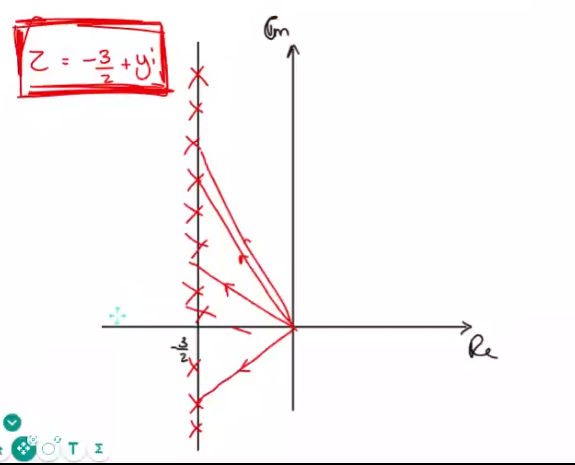
\includegraphics[scale=0.7]{ex1a complex loci}
		\end{center}
	\end{multicols}
	
	\begin{example}
		Given $\abs{\frac{z-1}{z+4i}} = 2 $ , find the locus of $z$.
	\end{example}
	Remembering: $\abs{\frac{z_1}{z_2}} = \frac{\abs{z_1}}{\abs{z_2}}$
	
	
	Let $z = x+yi$
	\begin{alignat*}{2}
		&                & \abs{\frac{z-1}{z+4i}} & = 2                   \\
		& \implies \quad & \abs{z-1}              & = 2\abs{z+4i}         \\
		& \implies \quad & \abs{(x-1)+yi}         & = 2\abs{x+(y+4)i}     \\
		& \implies \quad & \sqrt{(x-1)^2+y^2}     & = 2\sqrt{x^2+(y+4)^2} \\
		& \implies \quad & \sqrt{(x-1)^2+y^2}     & = 2\sqrt{x^2+(y+4)^2} \\
	\end{alignat*}
	\hrulefill
	\begin{example}
		Given that $z_A = \frac{1}{10} (-1+i)$ and $z_B = -\frac{1}{500} (11+127i)$ , find in the form a+bi the complex numbers $\frac{z_A}{z_B}$.
		If $P(x,y)$ is the point on the Argand diagram representing $z=x+yi$, determine the equation of the locus of $P$ where $\abs{z-z_A} = \abs{z-z_B}$.
	\end{example}
	$$\frac{z_A}{z_B}  =  \frac{1}{10} (-1+i) \div -\frac{1}{500} (11+127i)$$
	\begin{alignat*}{2}
		&   &                                     & =-5\cdot \frac{-1+i}{11+127i}                         \\
		&   &                                     & = \frac{5-5i}{11+127i} \cdot  \frac{11-127i}{11-127i} \\
		&   &                                     & = a+bi                                                \\
		&   & \therefore \quad a=-\frac{58}{1625} & ,\quad  b=-\frac{69}{1625}                            \\
		&   & \abs{z-z_A}                         & = \abs{z-z_B}                                         
	\end{alignat*}
	\newpage
	\begin{example}
		If the real part of $\dfrac{z+2}{z+2i}$ is equal to 1, show that the point $z$ lies on a straight line. Hence find the point $z_0$ on this line such that  $\abs{z_0} = \sqrt{2}$. Find also the quadratic equation with real coefficients which has $z_0$ as one of the roots.
	\end{example}
	
	Let $z = x+yi$\\
	\textbf{Showing that $\boldsymbol{z}$ lies on a straight line: }
	\begin{align*}
		&   & Re(\frac{z+2}{z+2i})           & = 1                                                                       \\
		&   & \implies \quad 1               & = Re(\frac{x+2+yi}{x+2i+yi})                                              \\
		&   & \implies \quad 1               & = Re\left(\frac{(x+2)+yi}{x+(y+1)i}\cdot \frac{x-(y+1)i}{x-(y+1)i}\right) \\
		&   & \implies \quad 1               & = Re\left(\frac{x(x+2) -i(y+2)(x+2) + iyx + y(2+y}{x^2 + (y+2)^2}\right)  \\
		&   & \implies \quad 1               & = \frac{x(x+2) + y(y+2)}{x^2 + (y+2)^2}                                   \\
		&   & \implies \quad x(x+2) + y(y+2) & = x^2  + y^2+4y+4                                                         \\
		&   & \implies \quad 2y              & = 2x-4                                                                    \\
	\end{align*}
	$$\therefore \quad y = x-2 \qed$$
	$$\text{Point } z \text{ lies on the straight line } y = x-2$$

	\begin{example}
		Shade on an Argand diagram the area represented by $\abs{z+i} < 4$.
	\end{example}~\\
	\setlength{\columnseprule}{0pt}
	\textbf{Finding the loci: }
	\begin{multicols}{2}
		\begin{center}
			\begin{align*}
				&   & \abs{z+i} & = \abs{x+(y+1)i}                                   \\
				&   &           & =\sqrt{x^2  + (y+1)^2}                             \\
				&   &           & =\sqrt{(x-0)^2 + (y-(-1))^2}                       \\
				&   &           & \text{ is the distance from point (0,-1) to (x,y)} 
			\end{align*}
		\end{center}
		\begin{center}
			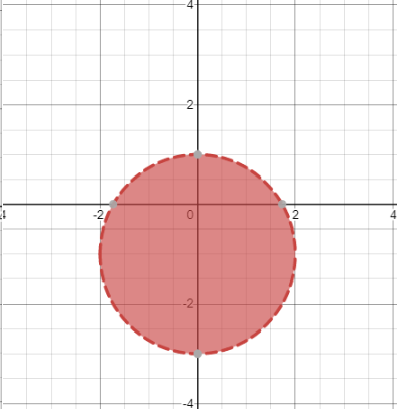
\includegraphics[scale=0.4]{complex_loci_ex5_circle}
		\end{center}
	\end{multicols}
	~\\~\\
\textbf{Finding $\boldsymbol{z_0= (a,b) = a+bi\colon}$}
	\reqnomode

			\begin{alignat*}{2}
			&               & z_0           & = a+bi       \\
			&\implies	&\abs{z_0}& = \sqrt{a^2+b^2}\\
			\intertext{Given:  $\abs{z_0}= \sqrt{2}$}
			& \implies\quad & \sqrt{a^+b^2} & = \sqrt{2}   \\
			& \implies\quad & a^2+b^2       & = 2\tag{1}   \\
			\intertext{We also know $z_0$ is on the line $y=x-2$}
	\therefore    b  = a-2\tag{2}	
			\intertext{Substituting 2 in 1: }
			&&a^2 + (a-2)^2 & = 2\\
			&\implies\quad&2a^2 - 4a+4 &= 2\\
		&\implies\quad &a^2-2a+1 &=0\\
		\end{alignat*}
		$$	\therefore\quad z_0 = 1-i \qed$$\\
\textbf{Finding quadratic equation with roots: $\boldsymbol{z_0, \bar{z_0}}$}
	\begin{center}
	$$x^2 - (\text{sum of roots})x + (\text{product of roots}) = 0$$
	$$\implies x^2 - (1-i + 1+i)x + (1-i)(1+i)=0$$
	$$\implies x^2-2x+2 = 0\qed$$
	\end{center}
\chapter{Applications of Calculus}
\section{Integrals}
\subsection{Volume of Revolution}

	If part	of a curve and the area underneath is rotated about a straight line, the solid formed is called a solid of revolution.\\

Consider the graph $y=f(x)$ and suppose we  rotate the part of the curve from $x=a$ to $x=b$ about the x-axis. If the shaded area of $f(x)$ is notated about the $x$-axis the following shape is formed:

	\begin{multicols}{2}
		\begin{center}
		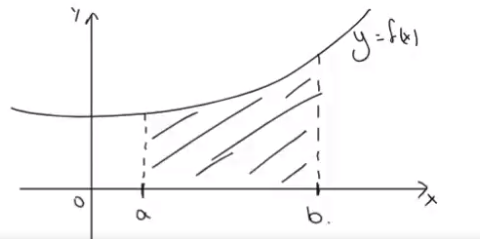
\includegraphics[scale=0.5]{app_of_calc_integ_1}
		\end{center}
	\begin{center}
		~\\
		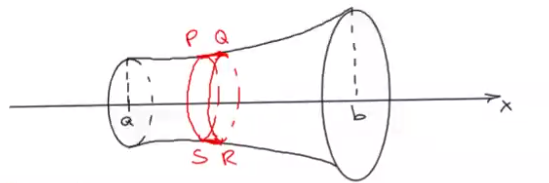
\includegraphics[scale=0.5]{app_of_calc_integ_2}
	\end{center}
	\end{multicols}


Suppose that the solid formed is cut into sections as shown. Let $PQRS$ be a typical section. If the cuts are reasonably close to each other, $PQRS$ approximates a cylinder with height $\delta x$ and radius $y$ as shown below:
\begin{center}
\qquad \qquad 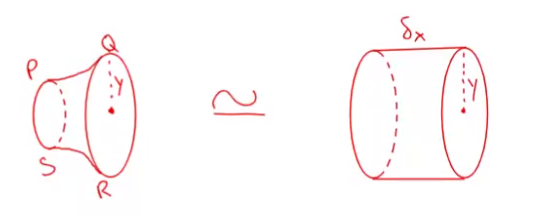
\includegraphics[scale=1]{app_of_calc_integ_3}
\end{center}
The volume, $\delta v$, of $PQRS$ is given by:
$$\delta V \simeq \pi y^2 \delta x$$
Thus, the volume $V$ of solid $PQRS$ is given by:
$$V\simeq \sum_{x=a}^{b} \pi y^2 \delta x$$
This summation approaches $V$ as $\delta x \to 0$
$$V = \lim\limits_{\delta x \to 0}   \sum_{x=a}^{b} \pi y^2 \delta x$$
$$\quad\boxed{V = \int_{a}^{b} \pi y^2 \, dx}$$
\hrulefill
\begin{example}
	Find the volume generated when the area  between $y=e^x$, the x-axis
\end{example}

\begin{alignat*}{2}
	&&V&=\int_{0}^{1} \pi y \, dx\\
\end{alignat*}

\begin{example}
	Find the volume generated when the area defined by the inequalities $y\leq x^2$ and $y\geq x$ is rotated about the $x$-axis.
\end{example}
\begin{multicols}{2}
	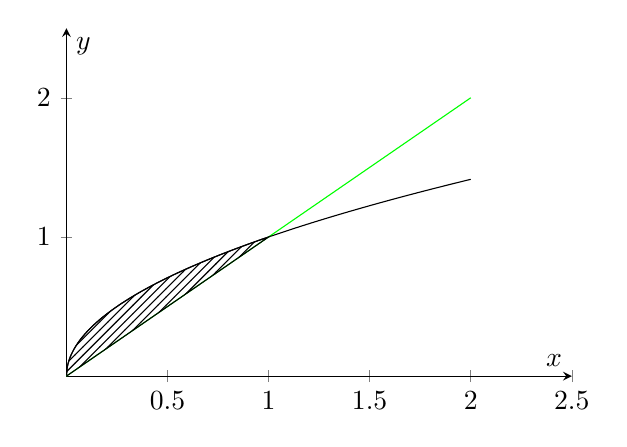
\begin{tikzpicture}
		\begin{axis}[
			width=8cm,
			height=6cm,
			axis line style={-},
			xmin=0,
			xmax=2.5,
			ymin=0,
			ymax=2.5,
			xtick={}, % remove all ticks from x-axis
			ytick={}, % ditto for y-axis
			xlabel=$x$, 
			ylabel=$y$,
			axis lines=center, % default is to make a box around the axis
			samples=100]
			\addplot [name path=A,samples=501, domain=0:2, black] {sqrt(x)};
			\addplot [name path=B,samples=501, domain=0:2, green]  {x};
			\draw[pattern=north east lines,
			intersection segments={
				of=A and B,
				sequence={L2--R2[reverse]}
			}];
		\end{axis}
	\end{tikzpicture}
\begin{center}
	
\end{center}

\end{multicols}
	\begin{alignat*}{2}
		&&	V_{e-c} &= V_e - V_c\\
		&&&= \pi \int_{0}^{1} \sqrt{x}^2 \, dx - \pi \int_{0}^{1} x^2 \, dx\\
	\end{alignat*}
\begin{example}
	Find the volume generated when the area in the first quadrant bounded by the circle $x=4\cos\theta, y=4\sin\theta$ rotates completely about the $x$-axis.
\end{example}
\begin{example}
	
	Find the volume when the region defined by  $y\geq x^+1,\quad x\geq0$ and $y\leq2$ is rotated about the $y$-axis.
\end{example}
	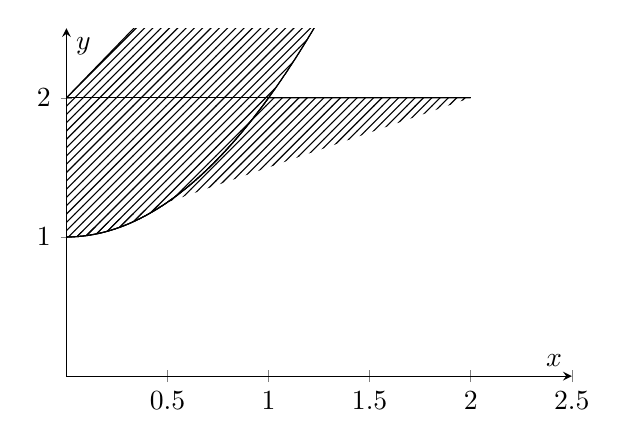
\begin{tikzpicture}
	\begin{axis}[
		width=8cm,
		height=6cm,
		axis line style={-},
		xmin=0,
		xmax=2.5,
		ymin=0,
		ymax=2.5,
		xtick={}, % remove all ticks from x-axis
		ytick={}, % ditto for y-axis
		xlabel=$x$, 
		ylabel=$y$,
		axis lines=center, % default is to make a box around the axis
		samples=100]
		\path[name path=axis] (axis cs:0,0) -- (axis cs:0,2);
		\addplot [name path=A, domain=0:2, black] {2};	
		\addplot [name path=B, domain=0:2, black]  {x^2 + 1};
		\draw[pattern=north east lines,
		intersection segments={
			of=axis and B,
			sequence={L2--R2[reverse]}
		}];
		\draw[pattern=north east lines,
		intersection segments={
			of=B and A,
		}];
	\end{axis}
\end{tikzpicture}


	\end{document}